\chapter{Diseño}

Éste apartado muestra una visión simplificada de como funciona la aplicación, será en la sección de implementación donde se completen los aspectos restantes cuya explicación resulta más fácil valiéndose del código usado además de las tecnologías con las que se llevan a cabo las tareas.

\section{Diseño del dispositivo receptor}

El dispositivo receptor tendrá instalado y en continua ejecución el módulo de reconocimiento de vehículos. Los elementos requeridos se detallaron en la sección \textit{presupuesto}.

\section{Diseño del módulo de reconocimiento de vehículos}
El lenguaje usado para la recepción de sonido será {\tt Python 3} debido a la facilidad de uso y el número de librerías que presenta. Por otra parte
El módulo principal estará compuesto de dos funciones usando como base un patrón típico en sistemas concurrentes, el  modelo de productor-consumidor. Ésto nos permitirá trabajar con dos hebras independientes (pero pertenecientes al mismo proceso) las cuales trabajan sobre una cola en la que la hebra productora va introduciendo los valores numéricos obtenidos por el micrófono mientras que el consumidor va extrayendo los mismos de la cola para su análisis, el cual se detalla en la subsección Desarrollos algorítmicos.

Una vez el consumidor ha concretado que la información recibida es indicador de que un vehículo ha pasado tiene dos tareas:

\begin{itemize}
  \item Enviar la información a la web mediante una petición POST que incluya un \textit{payload} con la información relativa al dispositivo como puede ser latitud, longitud, id del dispositivo, localización del dispositivo y número aproximado de vehículos que han pasado. Las peticiones serán aceptadas en el servidor web gracias a una api REST que atiende las peticiones de éste tipo.
  \item Transmitir la información al almacenamiento masivo mediante el soporte que nos provea la plataforma IOT seleccionada. La forma de proceder aquí es dependiente de cómo se interactúe con la plataforma por tanto los detalles de como el dispositivo envía la información en éste punto serán vistos en el sección de implementación.
\end{itemize}

\subsection{Estructuras de datos en el dispositivo receptor}
La estructura de datos más remarcable en éste módulo es la cola, sin duda es el elemento más apropiado para la recopilación y extracción de datos de manera simultánea. Además las colas en python están diseñadas para solventar problemas de tipo concurrente de manera interna.

\subsection{Desarrollos algorítmicos}

A continuación se explica cuál es la forma de proceder a la identificación de un vehículo mediante el sonido recogido, por eso es imprescindible hablar del análisis de señales además del algoritmo usado.

\begin{itemize}
  \item \textbf{Digitalización de señales: }

    \begin{itemize}
      \item Para obtener una señal discreta a partir de una señal continua, es decir, para convertir los datos del dominio del tiempo al dominio de la frecuencia nos valdremos de la transformada rápida de Fourier (FFT).
      \item Con los valores discretizados procedemos a multiplicarlos por una ganancia configurable mediante una constante, que ayudará a aumentar la señal o disminuirla dependiendo del tipo de micrófono que tengamos. Por último se suman los que pertenecen a un mismo bloque descartando aquellos que no entren dentro del rango de cuantización. Éste valor final es puesto en la cola sobre la que la hebra consumidora va extrayendo datos.
    \end{itemize}

  \item \textbf{Identificación de vehículos:} Una vez tenemos la suma de los valores para un bloque, en primer lugar comprobamos que la suma de ese bloque alcanza un nivel mínimo, éste nivel dependerá de las condiciones en las que se encuentre el dispositivo receptor. Por ejemplo, no es lo mismo que se encuentre situado en el primer piso de un edificio que en el tercero.

  Una vez tenemos filtrados los valores que superan ese mínimo es momento de contar cuantos bloques seguidos se obtienen por encima de esa cota. Al igual que hemos definido la cota mínima para considerar que existe un nivel de sonido perteneciente a un vehículo debemos definir el número de bloques consecutivos que necesitamos para considerar que un vehículo ha pasado y éste valor será dependiente de igual modo de las características de la carretera ya que el número de bloques necesarios para la identificación está estrictamente relacionado con la velocidad de los vehículos que circulan por la calle, es decir, cuanta más velocidad lleven menos bloques serán necesarios para proceder a la identificación del vehículo.

  El valor de cada bloque válido (que supera la cota), es almacenado en una cola, cuando el número de bloques es suficiente para concretar que un vehículo ha pasado los valores almacenados en la cola se mandan a la base de datos de almacenamiento masivo y ya estarán listos para su visualización.

  Para ilustrarlo con un ejemplo nos valdremos de la \textit{figura 5.1}.

  Cuando el vehículo pasa dentro del rango de captura del micrófono empiezan a contabilizarse los bloques con un valor superior a la cota definida desde \textbf{B1} hasta \textbf{BN}. Si tenemos un número de bloques válido contabilizaremos que ha pasado un vehículo. Si el número de bloques se ve interrumpido por 'silencio' o sonido por debajo de la cota, la contabilización de bloques se reinicia y en la cola de envío son descartados todos los elementos pertenecientes a los bloques consecutivos anteriores.
\end{itemize}
\begin{figure}[!ht]
  \begin{center}
    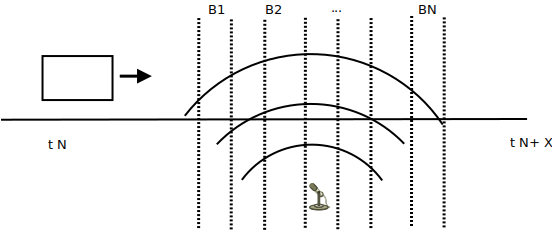
\includegraphics[scale=0.50]{../images/sound/soun_detect.png}
    \caption{Proceso de reconocmiento}
    \label{fig:recogn}
  \end{center}
\end{figure}

\section{Almacenamiento de información}

La información será enviada desde los dispositivos recolectores hasta el servidor que contiene la base de datos de almacenamiento masivo que se encontrará instalada en una instancia propia para garantizar que todos los recursos de la máquina se dedican a atender las peticiones de almacenamiento.

Ésta base de datos será de tipo NoSQL debido a que no se requiere ningún tipo de jerarquía sobre los datos y tampoco se precisa una estricta integridad de los mismos ni operaciones de tipo atómico.

\section{Representación de información}

Éste modulo también se encontrará en un servidor externo a los demás. En la configuración se establecerá la conexión hacia el servidor de almacenamiento masivo y a partir de ahí, se podrán lanzar consultas para obtener datos.

\section{Diseño del portal web}

El portal estará desarrollao con el framework Django, el cual hace uso del paradigma Modelo-Vista-Controlador por lo que tendremos por una parte la parte lógica o backend y por otro lado la parte visual o front-end. Tendrá la siguiente estructura de archivos y directorios:

\begin{itemize}
  \item \textbf{scripts}: contiene los scripts necesarios para automatizar tareas relativas a la web.
  \item \textbf{webapp}: contiene la aplicación web.
  \begin{itemize}
    \item \textbf{templates}: contiene las plantillas html de la web.
    \item \textit{apps.py}: archivo en el que se configura las aplicaciones instaladas de la web.
    \item \textit{models.py}: modelos de datos que serán usados.
    \item \textit{settings.py}: archivo de configuración general.
    \item \textit{urls.py}: definicióno de las rutas de la web.
    \item \textit{views.py}: definición de vistas
    \item \textit{wsgi.py}: configuración de despliegue.
  \end{itemize}
    \item \textit{manage.py}: encargado de ejecutar tareas de lanzar la aplicación además de actualizar los modelos de datos en la base de datos.
    \item \textit{requirements.txt}: dependencias necesarias para la aplicación.
    \item \textit{Makefile}: contiene la automatización de las tareas más comunes de la aplicación.
\end{itemize}

\subsection{Diseño de la api REST}

La api estará integrada dentro de Django gracias al módulo Django-Rest-Framework

TODO
